\documentclass{ximera}
%herschreven 13/11/26
\title{Het SI-stelsel en prefixen}
\author{Daan Lipkens}

\begin{document}
\begin{abstract}
    De zeven basiseenheden, afgeleide eenheden en het omzetten met prefixen en machten van 10.
\end{abstract}
\maketitle

\section{Het SI-stelsel}\label{sec:si_stelsel}
Het SI-stelsel legt voor zeven grootheden een \textbf{basiseenheid} vast (tabel~\ref{tab:si_basiseenheden}). Alle andere eenheden zijn daaruit opgebouwd.

\begin{table}[h]
    \centering
    \begin{tabular}{|l|l|c|}
        \hline
        \textbf{Grootheid} & \textbf{Basiseenheid} & \textbf{Symbool} \\
        \hline
        tijd & seconde & s \\
        lengte & meter & m \\
        massa & kilogram & kg \\
        elektrische stroomsterkte & ampère & A \\
        (absolute) temperatuur & kelvin & K \\
        hoeveelheid stof & mol & mol \\
        lichtsterkte & candela & cd \\
        \hline
    \end{tabular}
    \caption{De zeven basiseenheden van het SI-stelsel.}
    \label{tab:si_basiseenheden}
\end{table}

\begin{definition}[title={Afgeleide eenheid}]\nl
    Een \textbf{afgeleide eenheid} is een eenheid die je opbouwt uit basiseenheden, door ze met elkaar te vermenigvuldigen of door elkaar te delen. Je vindt ze uit de formule van de grootheid.
\end{definition}

\begin{example}[foldable=true,title={Voorbeeld: de eenheid van snelheid en van kracht}]\nl
    Bepaal de SI-eenheid van de gemiddelde snelheid $v = \dfrac{\Delta x}{\Delta t}$ en van de kracht $F = m \cdot a$.

    \begin{solution}\nl
        De verplaatsing $\Delta x$ druk je uit in meter, de tijd $\Delta t$ in seconde. Je deelt de eenheden dus ook door elkaar:
        \[ [v] = \frac{\mathrm{m}}{\mathrm{s}} = \mathrm{m/s} \qquad \text{(meter per seconde)} \]
        Voor de kracht vermenigvuldig je de eenheid van massa met die van versnelling:
        \[ [F] = \mathrm{kg} \cdot \frac{\mathrm{m}}{\mathrm{s^2}} = \mathrm{kg \cdot m/s^2} = \mathrm{N} \qquad \text{(newton)} \]
        De newton is dus geen basiseenheid, maar een afkorting voor $\mathrm{kg \cdot m/s^2}$.
    \end{solution}
\end{example}

\begin{question}
    Welke eenheid is \textbf{geen} SI-basiseenheid?

    \begin{multipleChoice}
        \choice{de kilogram}
        \choice{de ampère}
        \choice[correct]{de newton}
        \choice{de kelvin}
    \end{multipleChoice}

    \begin{solution}\nl
        De newton is een afgeleide eenheid: $1 \, \mathrm{N} = 1 \, \mathrm{kg \cdot m/s^2}$.
    \end{solution}
\end{question}

\section{Prefixen en machten van 10}\label{sec:prefixen}
De meter is handig voor de lengte van een lokaal, maar te klein voor de afstand tussen twee steden en te groot voor de dikte van een haar. Daarom zet je een \textbf{prefix} (voorvoegsel) voor de eenheid. Elke prefix staat voor een macht van 10 (tabel~\ref{tab:prefixen}).

\begin{table}[h]
    \centering
    \begin{tabular}{|l|c|c|l|}
        \hline
        \textbf{Prefix} & \textbf{Symbool} & \textbf{Macht van 10} & \textbf{Voorbeeld} \\
        \hline
        giga & G & $10^{9}$ & $1 \, \mathrm{GHz} = 10^{9} \, \mathrm{Hz}$ \\
        mega & M & $10^{6}$ & $1 \, \mathrm{MJ} = 10^{6} \, \mathrm{J}$ \\
        kilo & k & $10^{3}$ & $1 \, \mathrm{km} = 10^{3} \, \mathrm{m}$ \\
        hecto & h & $10^{2}$ & $1 \, \mathrm{hPa} = 10^{2} \, \mathrm{Pa}$ \\
        deca & da & $10^{1}$ & $1 \, \mathrm{dam} = 10^{1} \, \mathrm{m}$ \\
        -- & -- & $10^{0}$ & $1 \, \mathrm{m}$ \\
        deci & d & $10^{-1}$ & $1 \, \mathrm{dm} = 10^{-1} \, \mathrm{m}$ \\
        centi & c & $10^{-2}$ & $1 \, \mathrm{cm} = 10^{-2} \, \mathrm{m}$ \\
        milli & m & $10^{-3}$ & $1 \, \mathrm{mA} = 10^{-3} \, \mathrm{A}$ \\
        micro & $\mu$ & $10^{-6}$ & $1 \, \mathrm{\mu C} = 10^{-6} \, \mathrm{C}$ \\
        nano & n & $10^{-9}$ & $1 \, \mathrm{nm} = 10^{-9} \, \mathrm{m}$ \\
        \hline
    \end{tabular}
    \caption{De meest gebruikte prefixen. Boven kilo en onder milli gaan ze in stappen van $10^{3}$, tussen kilo en milli in stappen van $10$.}
    \label{tab:prefixen}
\end{table}

\begin{proposition}[title={Omzetten met machten van 10}]\nl
    \begin{itemize}
        \item \textbf{Naar de SI-eenheid:} vervang de prefix door zijn macht van 10. Bijvoorbeeld $3{,}5 \, \mathrm{mm} = 3{,}5 \cdot 10^{-3} \, \mathrm{m}$.
        \item \textbf{Van prefix A naar prefix B:} vermenigvuldig met $10^{a-b}$, met $10^{a}$ de macht van prefix A en $10^{b}$ die van prefix B. Bijvoorbeeld van km ($10^{3}$) naar mm ($10^{-3}$): $10^{3-(-3)} = 10^{6}$, dus $1 \, \mathrm{km} = 10^{6} \, \mathrm{mm}$.
    \end{itemize}
\end{proposition}

\begin{remark}[title={Controleer met je gevoel}]\nl
    Ga je naar een \emph{kleinere} eenheid, dan heb je er \emph{meer} van nodig: het getal wordt groter. Ga je naar een grotere eenheid, dan wordt het getal kleiner. Zo is $5 \, \mathrm{m}$ gelijk aan $5000 \, \mathrm{mm}$ en niet aan $0{,}005 \, \mathrm{mm}$.
\end{remark}

\begin{example}[foldable=true,title={Voorbeeld: kilometer naar meter en millimeter}]\nl
    Een loopwedstrijd is $5{,}4 \, \mathrm{km}$ lang. Druk deze afstand uit in meter en in millimeter.

    \begin{solution}\nl
        \begin{align*}
            5{,}4 \, \mathrm{km} &= 5{,}4 \cdot 10^{3} \, \mathrm{m} && \text{(prefix k vervangen door $10^{3}$)}\\
            5{,}4 \, \mathrm{km} &= 5{,}4 \cdot 10^{3-(-3)} \, \mathrm{mm} = \boxed{5{,}4 \cdot 10^{6} \, \mathrm{mm}} && \text{(van $10^{3}$ naar $10^{-3}$)}
        \end{align*}
    \end{solution}
\end{example}

\begin{example}[foldable=true,title={Voorbeeld: nanometer naar meter en micrometer}]\nl
    Groen licht heeft een golflengte van $530 \, \mathrm{nm}$. Druk deze golflengte uit in meter en in micrometer.

    \begin{solution}\nl
        \begin{align*}
            530 \, \mathrm{nm} &= 530 \cdot 10^{-9} \, \mathrm{m} = \boxed{5{,}30 \cdot 10^{-7} \, \mathrm{m}} && \text{(prefix n vervangen door $10^{-9}$)}\\
            530 \, \mathrm{nm} &= 530 \cdot 10^{-9-(-6)} \, \mathrm{\mu m} = 530 \cdot 10^{-3} \, \mathrm{\mu m} = \boxed{0{,}530 \, \mathrm{\mu m}} && \text{(van $10^{-9}$ naar $10^{-6}$)}
        \end{align*}
        Het getal wordt kleiner, want een micrometer is groter dan een nanometer.
    \end{solution}
\end{example}

\begin{remark}[expandable=true,title={Herhaling: de tabel uit de lagere school}]\nl
    Voor kleine stappen (m, dm, cm, mm) kan je ook de tabel gebruiken die je in de lagere school leerde. Je schrijft elk cijfer in een kolom, met de eenheid van je meetwaarde net voor de komma. Om $3{,}4 \, \mathrm{dm}$ om te zetten naar meter, schuif je de komma tot achter de kolom van de meter en vul je aan met nullen:
    \begin{center}
        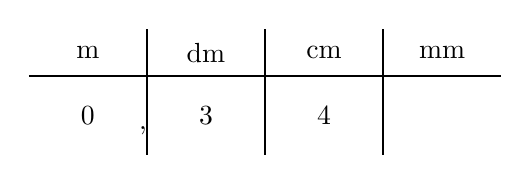
\begin{tikzpicture}
            \foreach \x in {0,1.5,3} \draw[thick] (\x,0) -- (\x,1.6);
            \draw[thick] (-1.5,1) -- (4.5,1);
            \foreach \eh/\x in {m/-0.75, dm/0.75, cm/2.25, mm/3.75} \node at (\x,1.3) {$\mathrm{\eh}$};
            \node at (-0.75,0.5) {0};
            \node at (0.75,0.5) {3};
            \node at (2.25,0.5) {4};
            \node at (-0.05,0.3) {,};
        \end{tikzpicture}
    \end{center}
    Zo vind je $3{,}4 \, \mathrm{dm} = 0{,}34 \, \mathrm{m}$. Bij grote stappen (micro, nano, mega, giga) wordt deze methode omslachtig: werk dan met machten van 10.
\end{remark}

\begin{question}
    Hoeveel meter is $1 \, \mathrm{\mu m}$?

    \begin{multipleChoice}
        \choice{$10^{6} \, \mathrm{m}$}
        \choice{$10^{-3} \, \mathrm{m}$}
        \choice[correct]{$10^{-6} \, \mathrm{m}$}
        \choice{$10^{-9} \, \mathrm{m}$}
    \end{multipleChoice}

    \begin{solution}\nl
        De prefix micro ($\mu$) staat voor $10^{-6}$, dus $1 \, \mathrm{\mu m} = 10^{-6} \, \mathrm{m}$: een miljoenste meter.
    \end{solution}
\end{question}

\end{document}
